% Template for PLoS
% Version 1.0 January 2009
%
% To compile to pdf, run:
% latex plos.template
% bibtex plos.template
% latex plos.template
% latex plos.template
% dvipdf plos.template

\documentclass[10pt]{article}

% amsmath package, useful for mathematical formulas
\usepackage{amsmath}
% amssymb package, useful for mathematical symbols
\usepackage{amssymb}

% for checkmarks
\usepackage{pifont}% http://ctan.org/pkg/pifont
\newcommand{\cmark}{\ding{51}}%
\newcommand{\xmark}{\ding{55}}%
% graphicx package, useful for including eps and pdf graphics
% include graphics with the command \includegraphics
\usepackage{graphicx}

% cite package, to clean up citations in the main text. Do not remove.
\usepackage{cite}

\usepackage{color} 

% Use doublespacing - comment out for single spacing
%\usepackage{setspace} 
%\doublespacing

%FZ: Enable the comment command
\usepackage{verbatim}
% Text layout
\topmargin 0.0cm
\oddsidemargin 0.5cm
\evensidemargin 0.5cm
\textwidth 16cm 
\textheight 21cm

% Bold the 'Figure #' in the caption and separate it with a period
% Captions will be left justified
\usepackage[labelfont=bf,labelsep=period,justification=raggedright]{caption}

% Use the PLoS provided bibtex style
\bibliographystyle{plos2009}

% Remove brackets from numbering in List of References
\makeatletter
\renewcommand{\@biblabel}[1]{\quad#1.}
\makeatother


% Leave date blank
\date{}

\pagestyle{myheadings}
%% ** EDIT HERE **


%% ** EDIT HERE **
%% PLEASE INCLUDE ALL MACROS BELOW
\long\def\authornote#1{%
        \leavevmode\unskip\raisebox{-3.5pt}{\rlap{$\scriptstyle\diamond$}}%
        \marginpar{\raggedright\hbadness=10000
        \def\baselinestretch{0.8}\tiny
        \it #1\par}}
\newcommand{\bastian}[1]{\authornote{BG: #1}}
\newcommand{\fabian}[1]{\authornote{FZ: #1}}
\newcommand{\philipp}[1]{\authornote{PB: #1}}
%% END MACROS SECTION
\begin{document}

% Title must be 150 characters or less
\begin{flushleft}
{\Large
\textbf{openSNP - a crowdsourced web resource for personal genomics}
}
% Alternative titles: 
% openSNP - a new, open data-source for personalised medicine
% What kind of person would share genotyping-data? Presenting a survey and an open data-source for personalised medicine
% 
% Insert Author names, affiliations and corresponding author email.
\\
Bastian Greshake$^{1,\ast}$, 
Philipp E. Bayer$^{2,3}$, 
Helge Rausch$^{4}$,
Julia Reda$^{5}$
\\
\bf{1} Molecular Ecology Group, Goethe University Frankfurt am Main, Germany
\\
\bf{2} School of Land, Crop and Food Sciences and Australian Centre for Plant Functional Genomics, University of Queensland, Brisbane, Australia
\\
\bf{3} Australian Centre for Plant Functional Genomics, School of Agriculture and Food Sciences, University of Queensland, Brisbane, Australia
\\
\bf{4} Hochschule f\"ur Technik und Wirtschaft Berlin, Germany 
\\
\bf{5} Johannes Gutenberg University Mayence, Germany
\\
$\ast$ E-mail: info@opensnp.org
\end{flushleft}

% Please keep the abstract between 250 and 300 words
\section*{Abstract}
Genome-Wide Association Studies are widely used to correlate phenotypic traits with genetic variants. These studies usually compare the genetic variation between two groups to single out certain Single Nucleotide Polymorphisms (SNPs) that are linked to a phenotypic variation in one of the groups. However, it is necessary to have a large enough sample size to find statistically significant correlations. Direct-To-Consumer (DTC) genetic testing can supply additional data: DTC-companies offer the analysis of a large amount of SNPs for an individual at low cost without the need to consult a physician or geneticist. Over 100,000 people have already been genotyped through Direct-To-Consumer genetic testing companies. However, this data is not public for a variety of reasons and thus cannot be used in research. It seems reasonable to create a central open data repository for such data.
%, but it was previously unknown if and how people would submit their data to such a repository.
%we present a survey which evaluates whether people are willing to publicly share their genetic information. In the light of those results 
Here we present the web platform openSNP, an open database which allows participants of Direct-To-Consumer genetic testing to publish their genetic data at no cost along with phenotypic information. Through this crowdsourced effort of collecting genetic and phenotypic information, openSNP has become a 
%valuable 
resource for a wide area of studies, including Genome-Wide Association Studies. openSNP is hosted at http://www.opensnp.org, and the code is released under MIT-license at http://github.com/gedankenstuecke/snpr


% Please keep the Author Summary between 150 and 200 words
% Use first person. PLoS ONE authors please skip this step.
% Author Summary not valid for PLoS ONE submissions.   
\section*{Author Summary}

\section*{Introduction}

The availability of new DNA sequencing techniques has shifted the focus of biological data acquisition towards new biomedical applications.
Many illnesses - for example Alzheimer's \cite{alzheimer}, Parkinson's \cite{parkinsons} or different types of cancers \cite{breastcancer,prostatecancer} - are at least partially heritable, so the genome of patients can be used for diagnostic purposes. Using the genetic information of patients for diagnostics is made possible through the sharp decrease in costs for analysing genetic information \cite{Brown1999}. 

%Kicked out the following due to Corpas' argument
%The comparison of DNA sequences from individuals in a population can reveal variable sites, which are of major interest in investigating diseases. 
%A variation of only one nucleotide length at a given site is called a single Nucleotide Polymorphisms (SNP). 
%The different nucleotides at this site are defined as an allele.
%For diploid organisms, as us humans, the genotype at a given site consists of two alleles, which are independently inherited from each parent.
%Different methods have been developed to read SNPs in an individual, a
%process called genotyping. A widespread used method for genotyping individuals is the use of microarrays.
%In comparison to whole genome sequencing only sites which are known to be variable are analysed, making microarrays cheaper and faster \cite{Brown1999}. 


If genetic information on more than one individual is known, the analysis of
allele frequencies of Single Nucleotide Polymorphisms (SNPs) can be used to associate such SNPs with illnesses and other inheritable traits. Genome-Wide Association Studies
(GWAS) make use of statistics to compare the allele frequencies in patients to the alleles in healthy controls. This
enables GWAS to find SNPs which are significantly overrepresented in patients and associates those SNPs with a trait or illness.
While method does not allow inference of causal differences but merely identifies correlations they can serve as a valuable tool for the unbiased discovery of candidate loci which then can be checked up in functional follow up studies \cite{10.1371/journal.pgen.1002584}, leading to a deeper understanding of diseases and thus potentially to new drug targets.  
The first GWAS was published in 2005 and compared age-related macular degeneration in contrast 
to a healthy control group \cite{Klein2005}. Since the beginning, the number of participants in 
such studies has been rising. To date, over 1200 GWAS have been performed \cite{Johnson2009} and over 
5000 SNPs have been linked to different illnesses and traits \cite{Hindorff2009}.   

GWAS are not only performed inside the traditional scientific community. 
Since 2006, companies like 23andMe, deCODEme or FamilyTreeDNA have been offering Direct-To-Consumer (DTC) genetic testing. 
These companies use DNA microarrays to screen for around 0.5 to 1 million SNPs spread over the human genome. In return, customers 
receive an analysis of the results, as well as a raw file that includes the customer's individual genotypes. In 2011, 23andMe 
alone had over 100,000 customers \cite{23andMe2011}
-- the company realizes the potential of performing GWAS with this amount of data by using surveys to ask their customers about 
traits and illnesses. With the consent of the customer, the data is used for association studies. 23andMe has published several 
studies in which known findings are replicated together with new associations for disorders like Parkinson's Disease \cite{Eriksson2010, Do2011}. 
So far, over 30,000 23andMe-customers have participated in 23andMe's association studies, which proves that this data source has a lot of potential for other researchers.

The generation of biomedical data by private companies raises concerns about privacy \cite{23andMe2012}, 
liability and consent \cite{Caulfield2011}. 
Nevertheless, in some instances individual customers are willingly sharing their data. Most do so by uploading their data to
their personal website or to open software repositories like \textit{GitHub}. 
This data is scattered and unorganized, making it hard to use in studies. While projects like SNPedia try to keep track of all 
the publicly available genotyping files \cite{Cariaso2011}, they usually do not provide the information necessary to perform GWAS, as the phenotypic information is 
often not attached to the genetic information. Projects that attach the phenotype to the genetic information, 
like the \textit{Personal Genome Project} \cite{Ball24072012}, still do not allow for an easy re-use of the data, as they currently lack an application programming interface (API) 
or other methods by which researchers could download the data. Additionally, not every customer of DTC genetic testing can participate in the \textit{Personal Genome Project}, as their consent forms only allow residents of the United States to apply.  

%Enter here: definition, benefits of sourcing
Crowdsourcing, giving a task into the hands of a potentially large number of -- mainly intrinsically motivated -- people, has become a widely used practice in the internet age and is getting adopted in the realm of science as well. One of the main benefits of crowdsourcing is that small contributions to a project pile up to create a larger work, which would have been virtually impossible to create otherwise. This approach especially benefits scientists who might not have enough funding or time to create data, or in cases where the amounts of data are too large to be analyzed by researchers alone.
 Galaxy Zoo and FoldIt \cite{Eiben2012, GalaxyZoo} are two of the best known examples. 
Galaxy Zoo enables amateur astronomers to walk through telescopic images to categorize the shown objects at a rate which could not have been matched by the efforts of professional astronomers.
Similarly, crowdsourcing can not only be applied to analyzing data, but also to collecting data. This approach has been shown to work when it comes to tracking bird migration \cite{CrowdsourcingReview2010}. With the advent of DTC genetic testing and the internet, a similar approach can now be applied to human genetics.

There have been studies investigating how likely customers of such companies are to share their data. \cite{Darst2013} investigated the likelihood of 2,024 individuals to share their test results with their health-care providers and found that 26.5\% (540 individuals) did share their results with their physician or health-care provider. Those that shared were older, had a higher income and were less concerned about testing or the privacy implications of sharing their data compared to customers that didn't share their data.

Other studies have shown that DTC-customers see themselves as being well-informed. Interviews with early adopters have shown that these customers are better informed and more skeptical about the capabilities of genotyping than expected \cite{McGowan2010}. However, in another study of early adopters, 32\% of customers had misperceptions about personal genomic testing \cite{Gollust2012}. Of these participants, 92\% intended to share their results with physicians in order to receive medical recommendations. In both studies, participants generally chose this technology to be better informed about genetic risks and to satisfy their own curiosity. 

Here, we present 
%the results of a survey designed to evaluate the support in the personal genetics community for a crowdsourced online platform. We also present 
openSNP, an online platform which enables DTC customers to share genotypic and phenoytypic information, as well as receive additional information on their genotypes. The genotypes are made available to researchers via the open Creative Commons Zero license.

% Results and Discussion can be combined.
\section*{Results}
%\subsection*{Survey on Sharing Genetic Information}
%In total 229 people, 180 with a self-reported chromosomal sex of XY and 56 with a self-reported chromosomal sex of XX, participated in our survey on sharing genetic information with the public. 
%The mean age of the participants is 33 (SD = 11,29). 81.7 \% reported their ethnicity as caucasian. 39.7 \% of the participants are already 
%customers of at least one DTC genetic testing company and further 30.1 \% of them plan on becoming one in the future. 29.7 \% do not plan on 
%becoming a DTC customer. There is no significant difference in the usage of DTC companies between chromosomal sexes (Cramer's V = 0.077). 
%
%67.7 \% of all participants would share their data with their DTC company without any constraints, 25.8 \% would do so given the company 
%didn't share the data with third parties. 6.6 \% of the participants would not share their data. Participants self-identified as XX-chromosomal are slightly more likely to answer that DTC companies are allowed to use their results (Cramer's V = 0.221). Those who are customers of a DTC company or are planning on becoming one in 
%the future are more likely to share their results, compared to those who do not plan on getting themselves genotyped (Somers-d = 0.331). 
%
%
%There are substantial differences in terms of motivation, tested by Tukey's HSD test, between those people who have already been genotyped 
%and those who are not planning on getting genotyped. The first group is likely to agree more strongly, on a five-point scale, with motivations for sharing genotypic information. On the other hand, those people who are not planning on getting genotyped are more likely to agree with the several motivations 
%for not sharing their data (for an overview of these motivations, see table \ref{tab:motivations1}).
%
%Similarly, those people who would share data with their DTC provider under any circumstances are likely to agree more strongly with 
%the following motivations for sharing than those who would not share their data with their DTC company.
%Those participants who are not willing to share data with their DTC company are likely to agree more strongly with some motivations 
%for not sharing their data when compared to those who would share their data with their DTC company under any circumstances. For an overview of the motivations of both groups, see table \ref{tab:motivations2}.
%
%In the case of curiosity as a motive, there is also a substantial difference between those who would share their data with their DTC company under the condition that it did not share the information and those who would not (mean difference = 1.116 SE = 0.344) as well as those who would share under any circumstances (mean difference = -0.874 SE = 0.182).
%
%In the cases of fear of discrimination and fear of a breach of privacy, substantial differences between all three categories exist. Those who would share their data with their DTC company as long as it did not share the information agree less strongly than those who would not share the data with both fear of discrimination as a motive for not sharing (mean difference = -0.615, SE = 0.345) as well as fear of a breach of privacy (mean difference = -0.668, SE = 0.346). Those who would share their data under any circumstances are even less likely to agree with these motives than those who would share only if their DTC company did not share the information (fear of discrimination: mean value = -0.906, SE = 0.182; breach of privacy: mean difference = -1.203, SE = 0.183).
%
%These survey results indicate that there is a definite interest in customers of DTC companies to share their results with other scientists. 

\subsubsection*{Sharing genotypic information}

We created the openSNP project (http://opensnp.org) as an open, crowdsourced online platform for DTC customers interested in sharing their raw data and for researchers interested in performing GWAS or other types of analysis with the data. 
Customers of DTC testing are encouraged to share their genotyping results along with their phenotypic traits to enable easy access for researchers.
Users of openSNP can create a personal profile, discuss SNPs and phenotypes on the platform using a simple commenting system, or send each other private messages.

People interested in using the data of openSNP can download complete dumps of the genotypic and phenotypic information or use query API endpoints utilizing JavaScript Object Notation (JSON) objects or the Distributed Annotation System (DAS) \cite{Dowell2001}. 


\subsection*{Sharing genotypic information}
Currently users can upload their genotyping results from the companies \textit{23andMe}, \textit{deCODEme} and \textit{FamilyTreeDNA} via a web interface to the openSNP 
project. There is experimental support for uploading exomes in the VCF format \cite{Danecek01082011}, as \textit{23andMe} recently started exome sequencing for its customers. Due to space constraints, openSNP currently only stores the SNPs of the exome data sets.
The uploaded data is published under the Creative Commons Zero license, 
which -- in accordance with the Panton Principles \cite{10.1371/journal.pbio.1001195} -- 
allows a complete re-use of the data without any constraints.
Between the launch of openSNP on 09/27/2011 and 10/27/2012, 633 people have signed 
up with openSNP, and 270 genetic datasets have been made available. As of 10/27/2012, the openSNP database lists 215,546,685 genotypes which are distributed over 2,140,643 unique SNPs.
Figures \ref{Figure1_label} and \ref{Figure2_label} depict the increase in users and genotyping files since September 2011.


\subsection*{Crowdsourcing phenotypes}
Users are able to create new phenotypes that are not yet 
listed by openSNP. 
The specification of these phenotypes is open and not limited 
to pre-defined categories. To reduce the amount of manual data curation, openSNP tries to harmonize 
the expression and spelling of the same phenotype or variation. We implemented an 
autocompletion feature, which helps users reuse already entered phenotypes.
Users are encouraged to list as many phenotypes as possible through a simple 
achievement system, rewarding users that upload their data and enter phenotypic 
information with badges that are shown on their profile pages.

In the same timeframe mentioned above, all users combined have 
entered a total of 4743 variations on 130 different phenotypes with those variations being 
the different values on a given trait or phenotype. The mean number of users that have entered their variations for a single phenotype 
is 36.48. The distribution of how many users have 
entered their data per phenotype, compared to the amount of unique phenotypes, can be seen in Figure \ref{pheno}. The phenotype provided by the most users is "eye color", for which 207 users entered their phenotype (retrieved 10/27/2012). 


\subsection*{Connection to external services}
In order to provide users with relevant information on their respective genotypes, openSNP scans databases of the scientific literature for specific SNPs. 
A total number of 21,134 documents relevant to the SNPs listed in openSNP could be found in the publication and annotation databases of Mendeley, the Public Library of Science, in the \emph{GET Evidence System} \cite{Ball24072012} and the \emph{NHGRI GWAS Catalog} \cite{Hindorff2009} and in the crowdsourced SNPedia (Figure \ref{Figure3_label}).
Of the primary literature listed on Mendeley, the \emph{NHGRI GWAS Catalog} \& the Public Library of Science, about 20 \% are released in open access journals and can be accessed free of charge (Figure \ref{oa_label}), although probably not all publications on Mendeley are correctly flagged and the \emph{NHGRI GWAS Catalog} does not give details on whether a publication is open access or not. So the total number of open access publications might be higher. 

For usability reasons, 
SNPs are ranked by the amount of information gathered through the external services. The external services themselves are ranked by how easily non-scientists can understand information 
from these sources and how available this information is to the public. The SNPedia entries are given the highest impact, as those are already manually curated and summarized in plain English, followed by open access publications out of 
the Public Library of Science and the curated databases of the \emph{GET Evidence System} and the \emph{NHGRI GWAS Catalog}. Lowest values are given to the Mendeley results, as the publications listed there are for the most part not freely available without subscriptions or one-time payments. 
An entry on SNPedia is valued 2.5 times as high as a PLOS publication or entries in \emph{GET} or the \emph{GWAS Catalog} and 5 times as high as a Mendeley entry. 

Users are also able to link their Fitbit\cite{fitbit} accounts to their user-accounts. Fitbit is a commercial service which lets its customers track their BMI, movement and sleep data. This data can be linked to openSNP to give interested researchers an automatically maintained dataset of body and sleep developments over time.

\subsection*{Data access}
openSNP offers complete access to the data uploaded by users. Anyone can download single genotyping files for specific users, get archives of multiple genotyping files 
grouped by phenotypic variation, or access a single download that includes all genotyping files and all phenotypic variation in a comma-separated table. For privacy reasons, openSNP does not log any IPs. The genetic data is also 
accessible through the Distributed Annotation System \cite{Dowell2001,Jenkinson2008}, which offers all data for specific chromosomes and specific positions on single chromosomes. 
An example of how the DAS can be used is implemented on openSNP, where users' genotypes are visualized inside a genome browser. All chromosomal positions are based on the human reference genome NCBI37, as this is the standard reference used by DTC providers right now.

The data is additionally available over a JSON API which allows users to directly access data in the JSON format. The methods allow users to programmatically look for the genotypes and annotations at a given SNP as well as for phenotypes for a given user and phenotypic variation for a given phenotype.

\section*{Discussion}

%\subsection*{Survey issues}
%
%As the survey was taken online by voluntary participants and was mainly spread in the personal genetics community, the results do not reflect the general population, but over-represent those people most likely to be interested in a project such as openSNP: customers of DTC genetic testing companies and people with a high interest in biology. 
%
Here, we present openSNP, a crowdsourced resource that enables customers of DTC testing companies to share their genotypings with researchers and receive new annotations for their genetic variants. With the number of active users already present on openSNP we have shown that customers of DTC companies are willing to share their data at no cost to researchers around the world and are willing to annotate their data with phenotypes.

\subsection*{Comparing openSNP to other crowdsourcing platforms}
Projects similar to openSNP are the SNPedia, the Personal Genome Project and PatientsLikeMe.com (see table \ref{tab:platforms} for an overview). The focus of the SNPedia is the aggregation and summary of primary scientific literature on SNPs. The project uses a Wiki to store and display the data collected by volunteers contributing to the project. The data is mainly organized by the unique Rs-ID, as given by dbSNP. If Rs-IDs are missing, the identifiers given by the DTC testing companies may be used, similar to the way openSNP stores the data. For individual SNPs, pages may list scientific literature and summaries on the found impact can be given. As those pages are largely created manually and not automatically through database access, these summaries may not be complete. openSNP utilizes the SNPedia by crawling their data for SNPs, the summary of the impact and the magnitude a SNP has. While they offer a page listing download-URLs, the SNPedia does not offer any uploading capabilities for genetic data and has no APIs to easily access SNPs or data subsets in the different data sets. Similarly, there is no way for users of SNPedia to share their phenotypes in a machine readable format. 

The Personal Genome Project (PGP) has its focus on collecting and hosting genetic as well as phenotypic data. Unlike openSNP, they do not offer a completely open enrollment. For each participant of the PGP, eligibility has to be established and participants have to give IRB approved informed consent. This allows for an easier re-use of the data, but at the same time makes it impossible for many people to enroll (e.g. non-US citizens). Depending on the specific use one has for the data, the PGPs enrollment policy might be preferable to the open approach openSNP takes. While the PGP stores genotyping data as well as exome and genome data sets, it is currently impossible to access this data through an API, instead data has to be manually extracted from their database. The annotation database of the PGP is not aimed at delivering specific publications, but instead focuses more on specific traits. The annotation data stored by the PGP is incorporated into openSNP as well. 

PatientsLikeMe is a community for patients with life-changing illnesses to track and share the development of their illness with other patients with similar illnesses \cite{Wicks2010}.  This helps patients in gaining a better understanding of their illnesses -- 72\% of surveyed participants found the site "moderately" or "very helpful", for example when it comes to starting a new medication (37\% found the site helpful), or when it comes to changing the medication (27\%). Some subsets of data stored in PatientsLikeMe are open to the public and have been shown to be useful for research, for example in Multiple Sclerosis \cite{Bove2013}. Alternatively, access to the data they store can be licensed by researchers for a fee. 

There are some projects that use gamification to let players work with crowdsourced scientific data. For example, FoldIt is a puzzle game that lets players fold protein structures in order to achieve optimal structures. Players of Foldit have been able to identify protein structures and were even able to improve the activity of existing protein structures \cite{Eiben2012}. Another example is Galaxy Zoo \cite{GalaxyZoo}, which allows everyone to perform classification tasks for galaxies based on images collected by the Sloan Digital Sky Survey. 

Unlike PatientsLikeMe, the PGP, or openSNP -- which give the task of collecting the data into the hands of the crowd -- Foldit and Galaxy Zoo limit themselves to analyzing data which was previously collected by scientists.  

\subsection*{Privacy, health implications and ethical considerations}

%The advent of DTC genetic testing has led to new ethical and social issues. 
Much of the criticism of DTC genetic testing focuses on the practice 
of delivering medical information without consulting a physician or genetic counselor to help patients/customers make sense of the information and to put the new knowledge to good use \cite{Hauskeller2011,Hogarth2008,Wasson2009}.  

%As we have found in our survey on sharing such results (see supplementary methods), many 
There is a variety of ethical and privacy implications when it comes to DTC genetic testing \cite{Caulfield2011,Joh2011,Joly2013}. But studies show that DTC customers are willing to share their results given the right circumstances and personal benefits gained through the sharing, while being aware that sharing genetic data can lead to misuse of the data and consequences like genetic discrimination  \cite{Darst2013}. 

%Our survey has shown that 
As people are concerned about their privacy and fear that stakeholders like employers, insurance companies, governments or advertisers might misuse the information \cite{Wolinsky2005}, policy makers start to react to those changes by having introduced laws like the 
\textit{Genetic Information Non-Discrimination Act} (GINA) in the United States or the \emph{Gendiagnostikgesetz} (GenDG) in Germany to minimize the impact of
widely available genetic information. DTC genetic testing companies themselves also try to create online communities - like the 23andMe community forums - that help in educating their customers about the risks of releasing genetic data \cite{Lee2009}. Neither GINA nor the GenDG offer a complete protection of genetic discrimination, as certain things, such as life insurances, are not covered by those laws.  

openSNP openly addresses the problem of privacy implications that come with releasing genetic data twice, once during registration for openSNP and once during 
the upload of the DTC genetic testing results. Users have to confirm that they have read and understood the disclaimer about possible side-effects 
of publishing their data. Further versions of openSNP may include further consent processes.

For users of openSNP the biggest potential problem is legal genetic discrimination in fields not covered by laws as GINA or GenDG once their public data is re-identified. While users can register pseudonymously this should not be seen as ultimate protection against re-identification. 
A recent study again showed that meta data, potentially attached to genetic profiles, such as date of birth, gender and postal code, can be be used to re-identify individuals on a name basis \cite{Sweeney2013}. 
A similar approach utilized genetic markers on the Y chromosome along with genealogical databases and meta data such as age and state to infer sure names and from there on the individuals \cite{Gymrek18012013}. 
Thus users need to be aware of the potential of re-idenification through providing meta data along with their genetic information and the genetic discrimination that could follow.

\subsection*{GWAS and Open Data}
Although prices of exome or even full genome sequencing are dropping rapidly, GWAS are still considerably cheaper. However, GWAS can only detect correlations of SNPs with those traits and do not allow 
inference on the cause for any correlation. Furthermore, for a statistically sound analysis, GWAS need a large enough sample size, which often is not easy to obtain. Either because generating the needed amount of data still is a cost factor or because it is hard to find enough participants for the case conditions, for example if rare diseases are to be studied. Nevertheless, GWAS are still frequently used and new associations are still being discovered \cite{10.1371.journal.pone.0031470,10.1371.journal.pone.0030309,10.1371.journal.pone.0029848}. 

One way of bringing down costs for GWAS even further is to make use of already available genotyping results and datasets. 
Data produced by DTC genetic testing companies is a promising source for such results, as those companies already have high 
numbers of customers which are willing to pay for the genotyping by themselves. 

openSNP tries to enable and facilitate the re-use of this already generated data by offering a platform where customers of DTC genetic testing can publish their results into the public domain. Allowing interested parties to use the data for their own research allows scientists to perform studies without the need to generate genetic data sets on their own. Additionally the data can be used to enrich other data sets in order to overcome limited sample sizes, which is especially of interest for rare diseases. 

In crowdsourcing the acquisition of genetic and phenotypic data, openSNP faces the same problems as any other 
open platform on the Internet, namely the need to trust users regarding the data they upload and enter on openSNP. 
Additionally, the quality of the data varies, especially in terms of accuracy on the phenotypic variation, 
with users entering data in different measurement systems. Another problem with user-entered data is the frequent switching between categorical and continuous phenotypes - for example, some users entered the specific value of their height, while other users entered their height according to a category like "150cm to 160cm". 

While we try to suggest similar entries to the users, 
there are some cases where users will not follow those suggestions, so duplicates or similar phenotypes or variations in traits may arise. There are three possible solutions to this problem: The first one would be to only allow a trusted subset of users to enter new phenotypes. The second one 
would be to make users enter all possible variations of a phenotype while creating a new phenotype, so that later users cannot add 
variations that have not been available from the start. The third one is to exclude users from the phenotype-creation process by allowing users to select their phenotypes from a pre-given set of possible variations.

In the first two cases it makes it harder 
for users to enter their data which raises the bar for participation, and the third case doesn't let users participate at all.
We decided to keep data entry as easy as possible, at the cost of forcing users who want to perform GWAS with the data to perform additional quality control.

Another risk regarding data quality that should be kept in mind is a possible bias in data availability on openSNP: only a subset of people buy DTC genetic testing, from which an even smaller subset is willing to publish the results, which can potentially lead to skewed GWAS-results. 21 people, mainly from underrepresented demographics, have been offered free genotypings using funding provided by the Wikimedia Germany association in order to mitigate this bias. 

Furthermore, it is impossible to verify whether users who have uploaded data are actually the sources of that data. This opens the venue to potentially malicious usage, as genotypings from strangers can be uploaded, as well as misinformation about phenotypes can be entered. The openSNP project has currently no means of verifying the validity of data uploaded by users. Of course, users can always delete their data or contact the team to delete stored data. Old backups of the database are deleted so that at any given time, there are only two backups. This means that deleted data disappears from the webpage immediately and will disappear after two months in the backend where it isn't accessible to the public.

With openSNP, we have built a platform that can be used by customers of DTC genetic testing to easily share their genetic and phenotypic 
data with a wide audience, as well as by scientists and interested citizens who are looking for datasets to freely use in their studies.
Customers of DTC genetic testing also benefit from an easy access to primary literature on SNPs and genetic variations they carry. 
While there is not enough data uploaded to perform a statistically sound GWAS yet, this will be possible in the future, as user numbers continue to rise. By including the option of uploading exome data sets, the platform is already capable of adjusting for changes in the type of data generated by DTC genetic testing. Future improvements made on openSNP will address interoperability with other platforms and tools in Personal Genomics, amongst others: The standardization of phenotypes, the inclusion of further annotation sources and support for a wider range of data sets, including full genome data.

 
% You may title this section "Methods" or "Models". 
% "Models" is not a valid title for PLoS ONE authors. However, PLoS ONE
% authors may use "Analysis" 
\section*{Materials and Methods}
\subsection*{Ethics Statement}
The director of the ethics commission of the Goethe University Frankfurt am Main, Germany teaching hospital confirmed that this study does not fall within their remit.

%\subsection*{Survey on Sharing Genetic Information}
%The survey was performed using \textit{Google Docs} and was distributed to possible participants through the \textit{23andMe }community forums, the \textit{DIYBiology} mailing list, 
%blogs which focus on genetics and DTC genetic testing and social media websites like \textit{Twitter}, \textit{Google+} and \textit{Facebook}.  
%
%The survey included demographics such as age, chromosomal sex and ethnicity of the participants. Furthermore, it included questions on their 
%(planned) customership with a DTC company. If the participants already were customers, they were also asked if they were already sharing their genetic and phenotypic data. 
%All participants were asked if they would be willing to share their genetical or phenotypic information with their DTC company, possible answers were "Yes", "Yes, 
%but only if they did not share my medical information with anybody else" and No".
%
%The survey also asked some scaled questions, which measured how strongly participants agreed/disagreed with different reasons for sharing or not sharing their 
%information. The scale went from 1 = strongly disagree to  5 = strongly agree. Motivations queried for sharing data 
%were "because I want to help scientists with their research", "because of possible personal benefits (e.g. getting treatments for a disease I have, 
%possibility of new medication, etc.)", "because it may deliver advertising that is relevant to me" and "out of curiosity". Motivations queried for not sharing 
%data were "because advertisers could use the information for targeted campaigns", "because of possible negative consequences for closely related persons", 
%"because of the breach of my privacy" and "because of the fear of discrimination (e.g. by the employer, the state, some insurance company)". 
%Additionally, participants had the possibility of giving their own reasons for sharing or not sharing their data.
%
%The survey data was analyzed with SPSS 19. 

\subsection*{Technical implementation of the platform}
The main platform is implemented using the web framework Ruby on Rails 3.2.13. Postgres 9.2 is used as the main database backend for Rails. 
The database stores genotyping results, users' phenotypic information, literature results from Mendeley and the Public Library of Science as well as summaries on SNPs 
which can be found in SNPedia. The literature database of Mendeley is queried using the REST API, which delivers results in JSON. The literature database of 
the Public Library of Science is queried using the respective REST API, which delivers results in an XML-format. Summaries on SNPs are provided by SNPedia, 
through querying the content via the MediaWiki API. The \emph{NHGRI GWAS Catalog} and the \emph{GET Evidence System} provide complete dumps in plain text formats. Those are regularly downloaded and parsed. SNPs that are described as 'Insufficiently evaluated' in the \emph{GET Evidence System} are not stored. All databases are queried or parsed using the unique identifier of each SNP as the search term. 

SNPs are catalogued by their unique identifier, which consists of a prefix (mostly \textit{rs}, rarely \textit{i}) and a unique number. This is a common format, 
which is employed by the NCBI dbSNP database \cite{Sherry2001} and is also widely used and easily parsed from different literature sources. Publications from the different databases as 
well as the users' genotypes are associated with individual SNPs by the Rs-ID. Allele and genotype frequencies are updated regularly, based on the data present in openSNP. 

Processes with a longer runtime, such as parsing the genotyping results, creating archives of results which are to be mailed to users and queries to external resources 
are handled using the ruby gem Resque and the standalone key-value storage server Redis. Search features on the platform itself are implemented using Solr and the ruby gem Sunspot. 
Additionally, data can be requested from openSNP using the Distributed Annotation System. The required data is stored in a PostgreSQL database.  
Requested data is delivered in XML-format to facilitate parsing. Additionally, users can request data in the JSON-format, using a system not specified in any standard.

openSNP only serves as a platform for SNPs, so methods for the delivery of nucleotide sequences as described in the DAS-standard are not implemented. Currently, 
two methods are implemented: firstly \textit{features}, which is used to deliver SNPs located on specific chromosomes or between specific nucleotide positions, 
based on the user's query. The second method is \textit{sources}, which advertises all DAS sources for all genotypes present in openSNP.

A flowchart of all services incorporated in openSNP and of all the ways users can upload or access the data is given in Figure \ref{Figure4_label}. The source code of openSNP is 
published under the MIT license and can be downloaded at http://github.com/gedankenstuecke/snpr. The genetical and phenotypical data is licensed under Creative Commons Zero. 
% Do NOT remove this, even if you are not including acknowledgments
\section*{Acknowledgments}
We thank Dr. Manuel Corpas and Prof. David Edwards for constructive advice in grammar, spelling and structure of this study. Further thanks go to Samantha Clark, Fabian Zimmer and Dan Bolser for providing valuable feedback and feature ideas during the development and Thomas Down, author of \emph{BioDalliance}, and Rafael Jimenez, author of \emph{MyKaryoView}, for their support on implementing the Distributed Annotation System and the genome browser. For help with their APIs we are grateful to Mike Cariaso of \emph{SNPedia} and the PLOS \& Mendeley API teams. Thanks go to Misha Angrist and the anonymous reviewers for their helpful comments on this manuscript. We would especially like to thank the users of openSNP.org for their participation, their constructive criticism and bug-finding abilities and especially for sharing their genotyping and phenotype data.

%\section*{References}
% The bibtex filename
\bibliography{papers}

\section*{Figure Legends}
\begin{figure}[!ht]
	%\begin{center}
	%	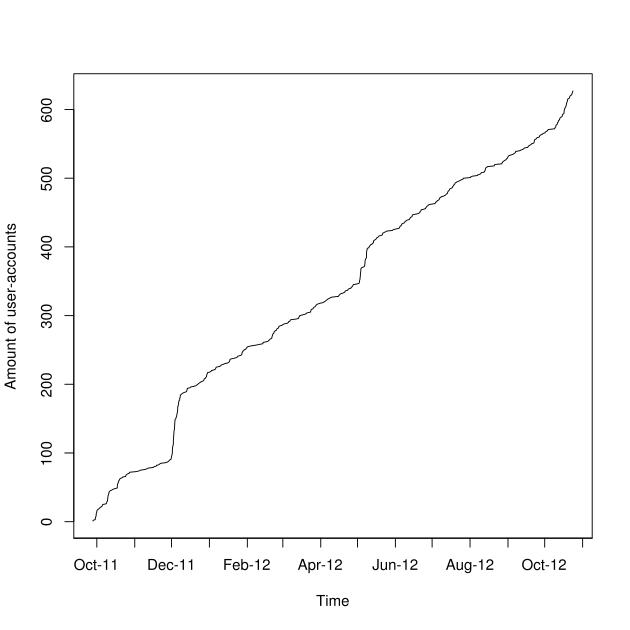
\includegraphics[scale=0.35]{25_10_2012_Graphs/users.png}
	%\end{center}
	\caption{
	{\bf Growth of openSNP-user-accounts.} The increase in numbers for users from 27.09.2011 to 27.10.2012 is shown.} 
	\label{Figure1_label}
\end{figure}
\begin{figure}[!ht]
	%\begin{center}
	%	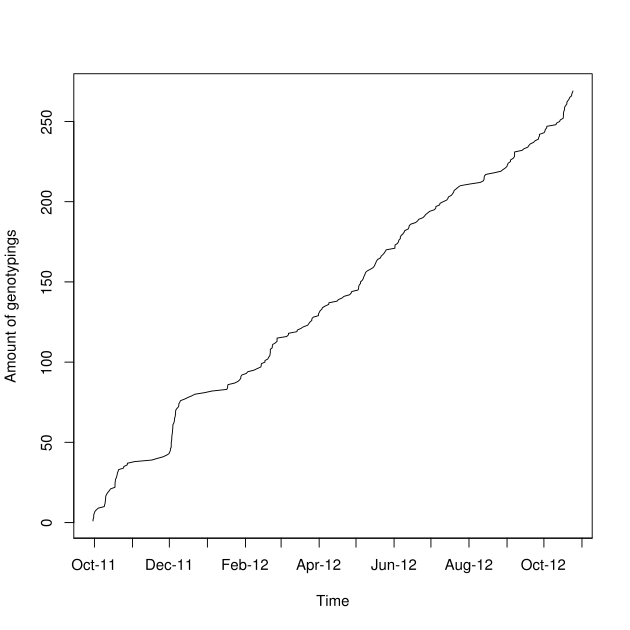
\includegraphics[scale=0.35]{25_10_2012_Graphs/genotypes.png}
	%\end{center}
	\caption{
	{\bf Growth of available genotypings.} The increase in numbers for genotyping-files from 27.09.2011 to 27.10.2012 is shown.} 
	\label{Figure2_label}
\end{figure}
\begin{figure}[!ht]
	%\begin{center}
	%	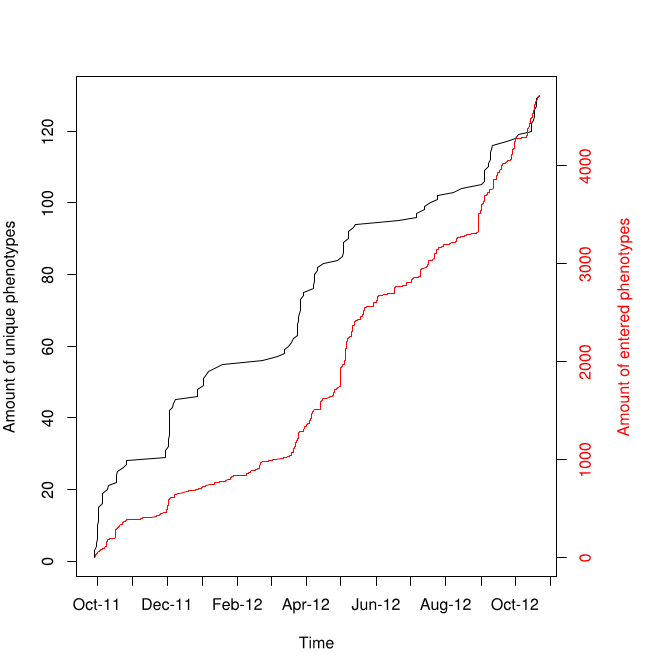
\includegraphics[scale=0.40]{25_10_2012_Graphs/phenotypes_vs_userphenotypes.png}
	%\end{center}
	\caption{
	{\bf Development of unique phenotypes and phenotypic information over time.} The x-axis shows the time-frame from start of the project until October 2012, the left y-axis shows how many unique phenotypes have been entered, and the right y-axis shows the amount of phenotypes users entered.}
	\label{pheno}
\end{figure}

\begin{figure}[!ht]
	%\begin{center}
	%	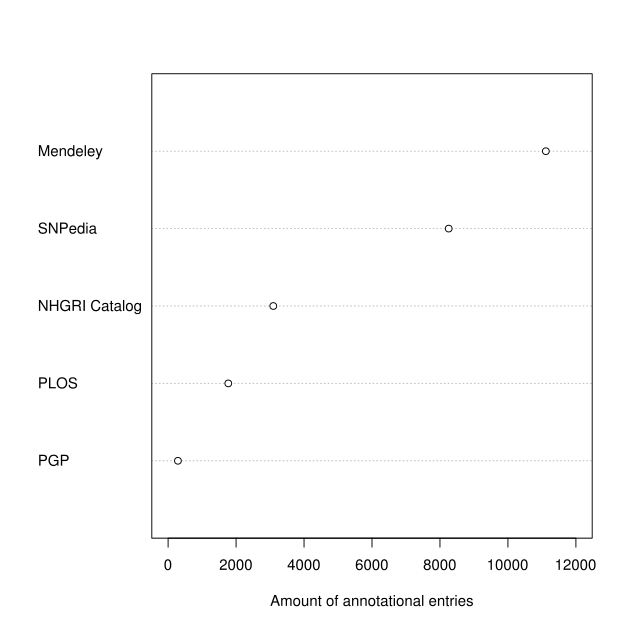
\includegraphics[scale=0.5]{25_10_2012_Graphs/papers_dotchart.png}
	%\end{center}
	\caption{
	{\bf Distribution of annotation-sources at openSNP.} Currently, SNP-annotations from SNPedia, PLOS, Mendeley, the \emph{GET Evidence System} and the \emph{NHGRI GWAS Catalog} are being collected.}
	\label{Figure3_label}
\end{figure}

\begin{figure}[!ht]
	%\begin{center}
	%	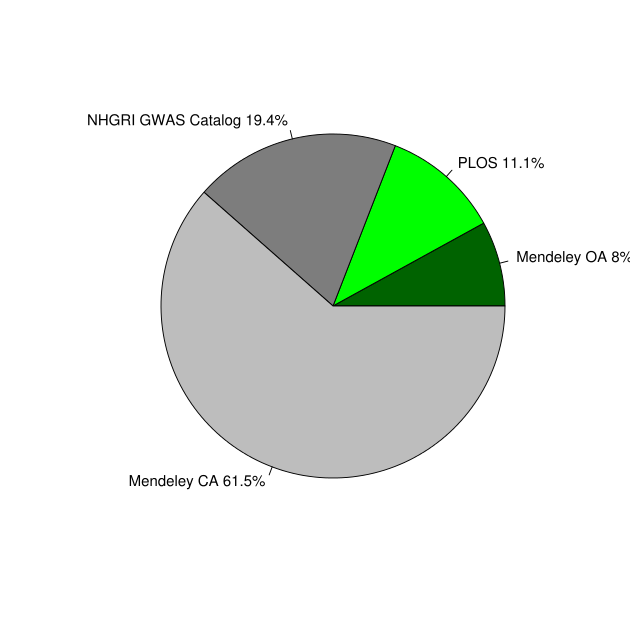
\includegraphics[scale=0.6]{25_10_2012_Graphs/new_pie.png}
	%\end{center}
	\caption{
	{\bf Ratio of open access Publications.} Green pieces are open access. The \emph{NHGRI GWAS Catalog} doesn't give information about the open access status.}
	\label{oa_label}
\end{figure}

\begin{figure}[!ht]
	%\begin{center}
	%  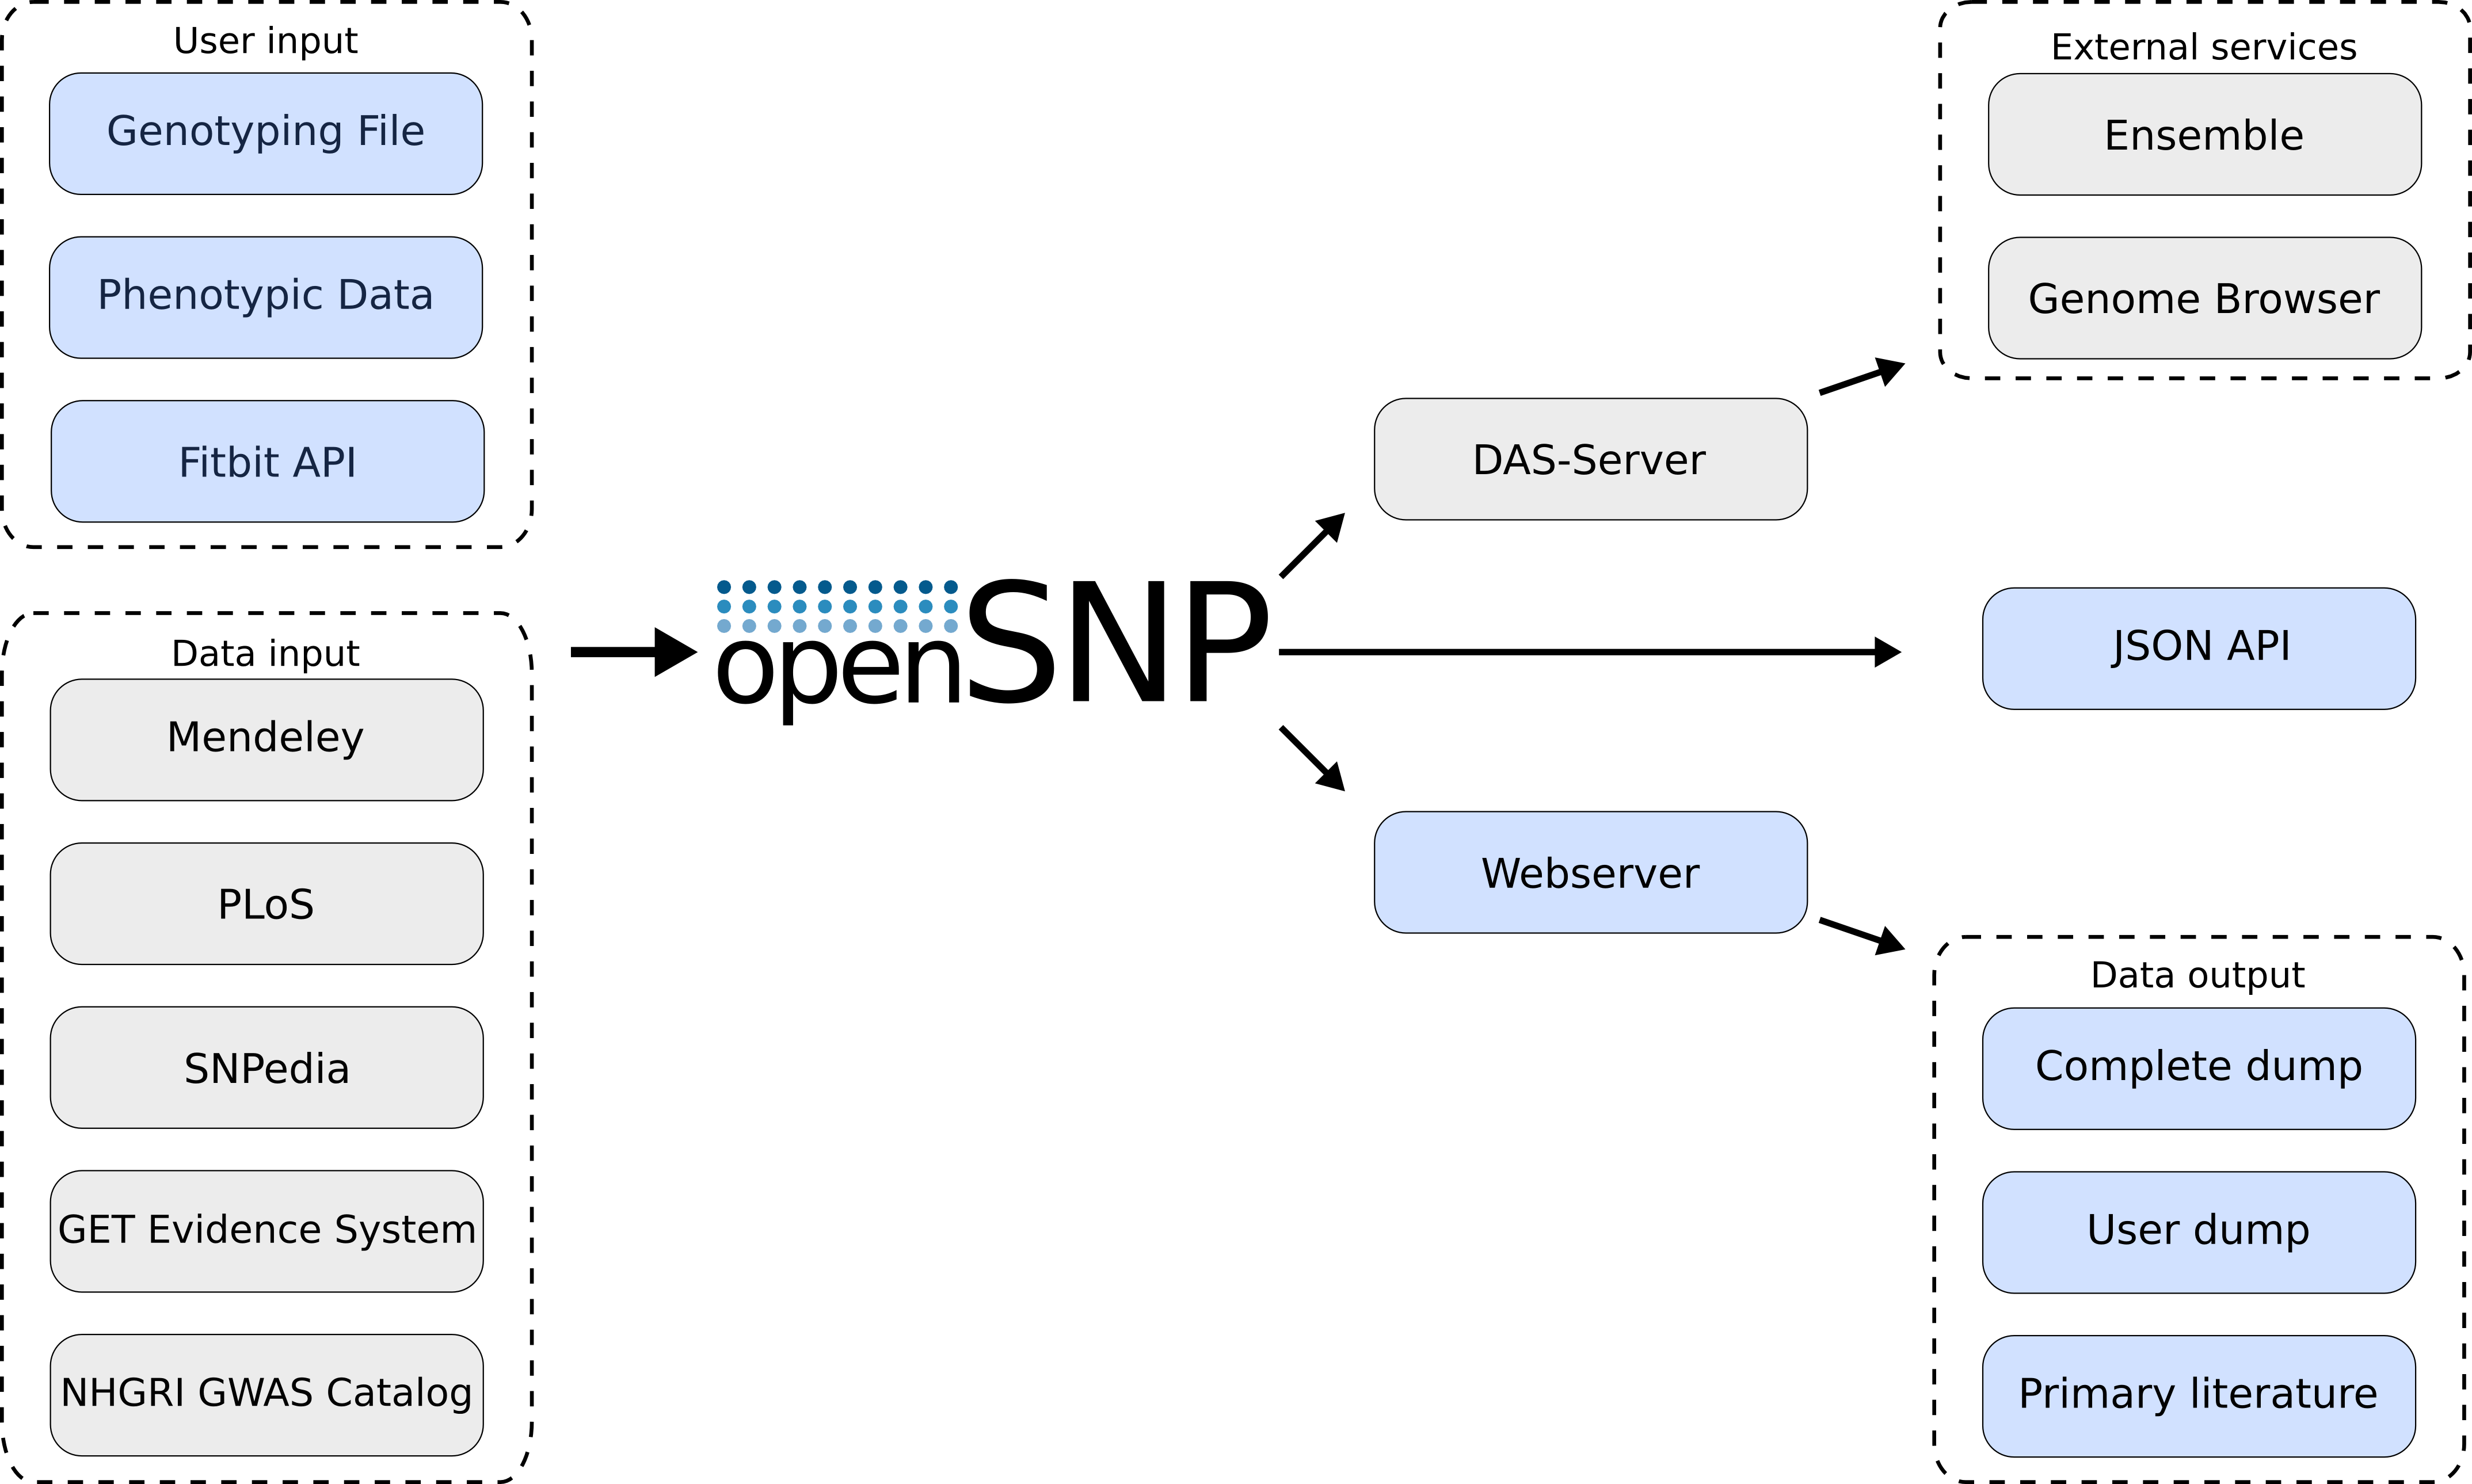
\includegraphics[scale=0.3]{latest_uml.png}
	%\end{center}
	\caption{
	{\bf Flow of data inside openSNP.} External databases and user-provided data are used as input. Output of data is done using the website, the \emph{Distributed Annotation System} and a JSON-API.} 
	\label{Figure4_label}
\end{figure}



%\begin{figure}[!ht]
%\begin{center}
%%\includegraphics[width=4in]{figure_name.2.eps}
%\end{center}
%\caption{
%{\bf Bold the first sentence.}  Rest of figure 2  caption.  Caption 
%should be left justified, as specified by the options to the caption 
%package.
%}
%\label{Figure_label}
%\end{figure}


\section*{Tables}
\begin{table}
\caption{Comparison of crowdsourced genetics platforms. N/A = Not Applicable, \checkmark = Present, \xmark = Absent}
\begin{tabular}{|l|l|l|l|l|l|l|}
\hline
Name & Provides  & Provides & Open  & API & IRB approval & License \\ 
& annotation & data & enrollment & & & \\
\hline
SNPedia & \checkmark & \xmark & N/A & \checkmark & N/A & CC-NC-SA 3.0 \\ 
\hline
PGP & \checkmark & \checkmark & \xmark & \xmark & \checkmark & CC-BY 1.0, CC0 \\
\hline
PatientsLikeMe & \xmark & \checkmark & \checkmark & \xmark & \checkmark & Closed, CC-BY-SA 3.0 \\
\hline
openSNP & \checkmark & \checkmark & \checkmark & \checkmark & \xmark & CC-BY 3.0 \\
\hline
\end{tabular}
\label{tab:platforms}
\end{table}
%\begin{table}
%\caption{Differences in terms of motivation to share genotypings with the public in survey-participants who already received a genotyping compared to participants who are not planning to getting genotyped. }  
%\begin{tabular}{|p{7cm}|p{2cm}|p{2cm}|p{2cm}|p{2cm}|}
%\hline
%& Mean \emph{Genotyped} & Mean \emph{Not Genotyped} & Mean Difference & Standard Error\\ 
%\hline
%\textbf{Motivation for sharing data in participants who are already genotyped} & & & & \\
%\hline 
%... curious & 3.82 & 2.66 & 1.159 & 0.193 \\ \hline % checked
%... want to help scientists & 4.64 & 4.18  & 0.465 & 0.128 \\ \hline % checked
%... for personal benefits & 3.77 & 3.32  & 0.448 & 0.183 \\ \hline % checked
%\textbf{Motivation for not sharing in participants who are not planning to get genotyped} & & & & \\ \hline
%... fear of discrimination & 3.09 & 4.15  & 1.06 & 0.195 \\ \hline % checked
%... breach of privacy & 3.01 & 3.68  & 0.666 & 0.211 \\ \hline % checked
%... fear of personalized advertising & 3.03 & 3.88  & 0.848 & 0.208 \\ \hline % checked
%... negative consequences for family members & 2.93 & 3.57  & 0.639 & 0.197 \\ \hline 
%\end{tabular}
%\label{tab:motivations1}
%\end{table}
%
%\begin{table}
%\caption{Differences in terms of motivations to share genotyping-data, comparison between participants who would share their genotyping data with participants who would not share their data.}
%\begin{tabular}{|p{7cm}|p{2cm}|p{2cm}|p{2cm}|p{2cm}|}
%\hline
%& Mean {Sharing} & Mean {Not Sharing} & Mean Difference & Standard Error \\ 
%\hline
%\textbf{Motivation for sharing genotypings in participants who would share} & & & & \\
%\hline
%... curiosity & 3.86 & 1.87 & 1.99 & 0.321 \\ \hline % checked
%... want to help science & 4.70 & 3.13 & 1.57 & 0.199 \\ \hline % checked
%... for personal benefits & 3.68 & 2.73 & 0.951 & 0.308 \\ \hline % checked
%\textbf{Motivation for sharing genotypings in participants who would not share} & & & & \\
%\hline
%... fear of discrimination & 3.21 & 4.73 & 1.52 & 0.322 \\ \hline % checked
%... fear of consequences for family members & 2.79 & 3.93 & 1.146 & 0.32 \\ \hline % checked
%... fear of personalized advertising & 3.17 & 4.29 & 1.112 & 0.357 \\ \hline % checked
%\end{tabular}
%\label{tab:motivations2}
%\end{table}
%\begin{table}[!ht]
%\caption{
%\bf{Table title}}
%\begin{tabular}{|c|c|c|}
%table information
%\end{tabular}
%\begin{flushleft}Table caption
%\end{flushleft}
%\label{tab:label}
% \end{table}

\end{document}
